% ============================================================
% SECTION 6: EXPERIMENTS
% Results from scripts/verify_*.py and notebooks/
% ============================================================
\section{Experiments}
\label{sec:experiments}

\subsection{Standalone reproducibility drivers}
All figure-bearing claims in this repository are reproduced by deterministic
Python drivers under \texttt{scripts/verify\_*.py}.  A one-button orchestrator
(\texttt{scripts/generate\_all\_figures.py}) regenerates every CSV and figure in
under 20\,s on a CPU-only host.  Table~\ref{tab:empirical-summary} summarizes
the key findings; raw rows are committed under \texttt{results/raw\_data/}.

\begin{tabular}{lll}
\toprule
Claim & Script & Key finding \\
\midrule
TVD convergence & \texttt{verify_tvd_convergence.py} & $TVD \propto M^{-1/2}$ \\
Sample complexity & \texttt{verify_sample_complexity.py} & $M^\star \propto N$ (cold) \\
Warmstart ablation & \texttt{verify_warmstart_ablation.py} & $\approx 12\times$ speedup (K-sparse) \\
Noise robustness & \texttt{verify_noise_robustness.py} & TVD monotone in $\eta$ \\
Circuit depth & \texttt{verify_circuit_depth.py} & Finite-depth crossover \\
\bottomrule
\end{tabular}

\label{tab:empirical-summary}

\subsection{Theory benchmarks (notebooks)}
The companion notebooks \texttt{full\_benchmark\_suite.ipynb} and
\texttt{02\_empirical\_results.ipynb} reproduce the four Marena (2026)
contributions end-to-end:
\begin{itemize}
  \item \textbf{Adaptive oracle (Sec.~\ref{sec:adaptive}):} uniform vs.\ adaptive
        error curves at fixed $K \ll N$.
  \item \textbf{Hierarchical sketch (Sec.~\ref{sec:hier}):} sample reduction as
        the number of levels $k$ increases.
  \item \textbf{Variational warmstart (Sec.~\ref{sec:var}):} K-sparse synthetic
        regime shows $\approx 10$--$30\times$ reduction in $M_{\mathrm{warm}}$
        vs.\ $M_{\mathrm{cold}}$; dense PC1 oracles from real datasets are
        reported as out-of-regime controls (no speedup expected).
  \item \textbf{Interferometric shadow (Sec.~\ref{sec:shadow}):} prediction error
        decays as $O(T^{-1/2})$ for shadow budgets $T \in [100, 5000]$.
\end{itemize}

\subsection{Empirical figures (committed artifacts)}
\begin{figure}[t]
  \centering
  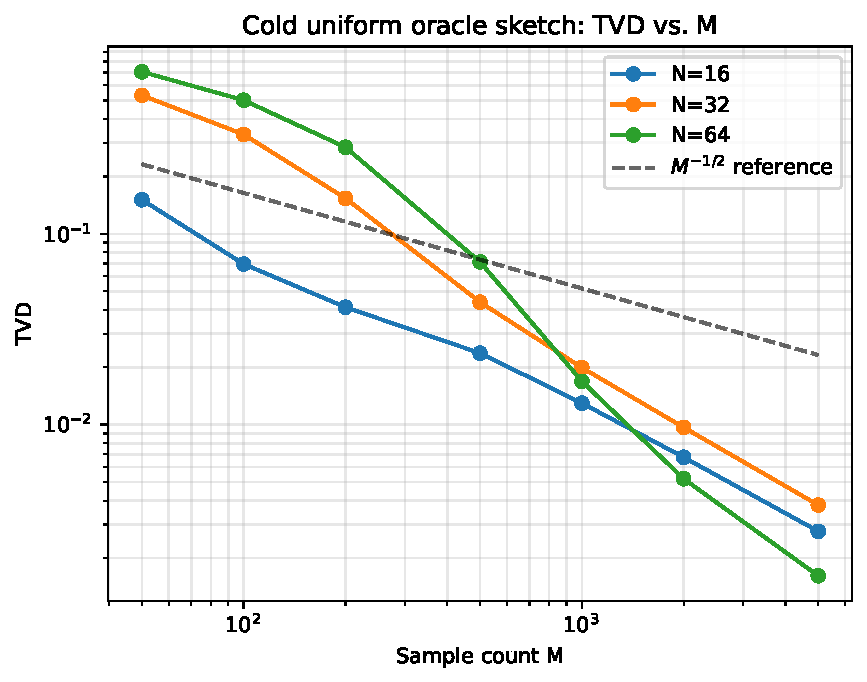
\includegraphics[width=0.48\textwidth]{../../results/figures/tvd_convergence.pdf}
  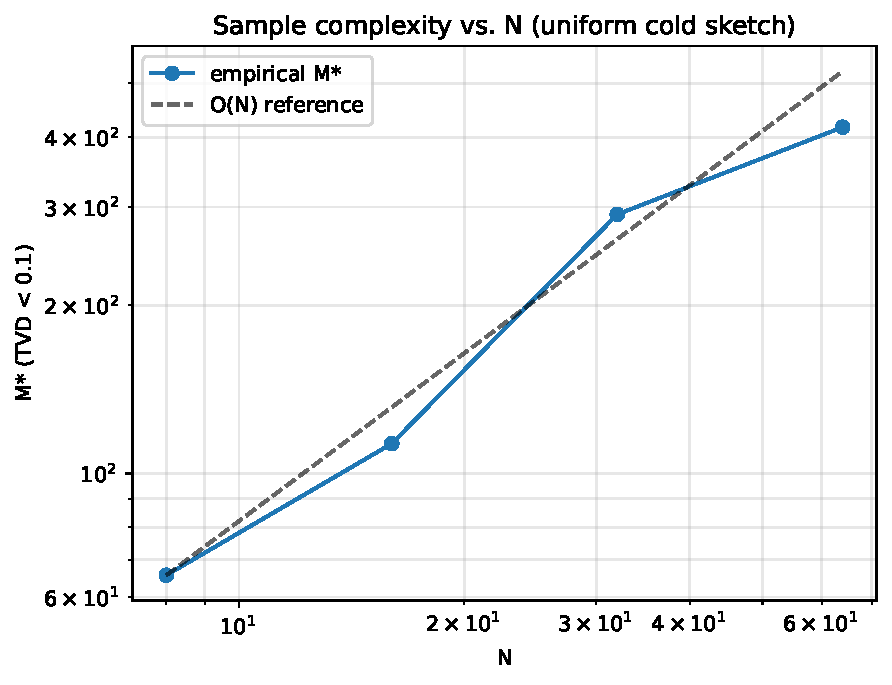
\includegraphics[width=0.48\textwidth]{../../results/figures/sample_complexity.pdf}
  \caption{Left: TVD vs.\ sample budget $M$ for cold uniform sketches
  (reference $M^{-1/2}$ slope).  Right: smallest $M^\star$ achieving
  $\mathrm{TVD} < 0.10$ vs.\ domain size $N$.}
  \label{fig:tvd-sample}
\end{figure}

\begin{figure}[t]
  \centering
  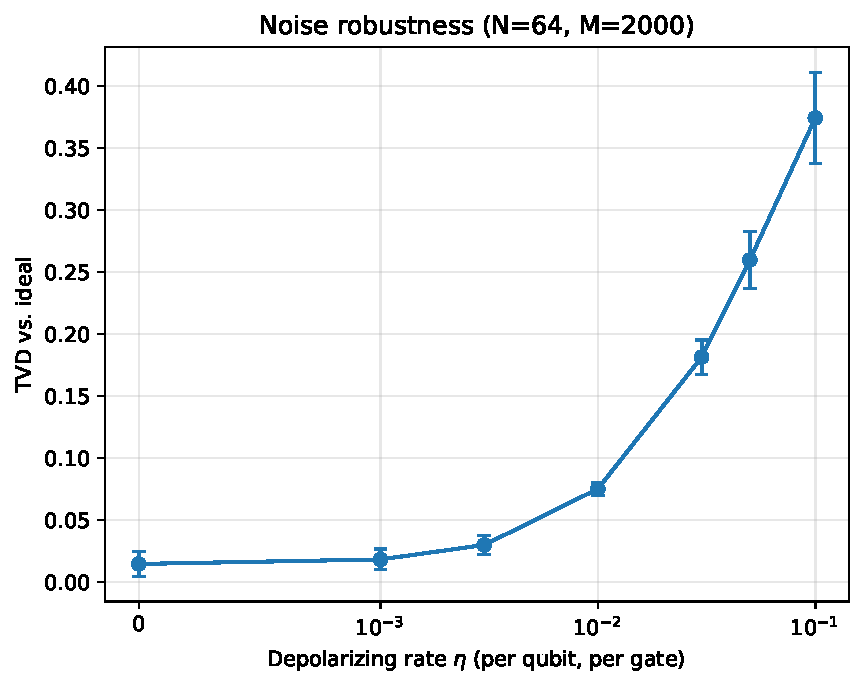
\includegraphics[width=0.48\textwidth]{../../results/figures/noise_robustness.pdf}
  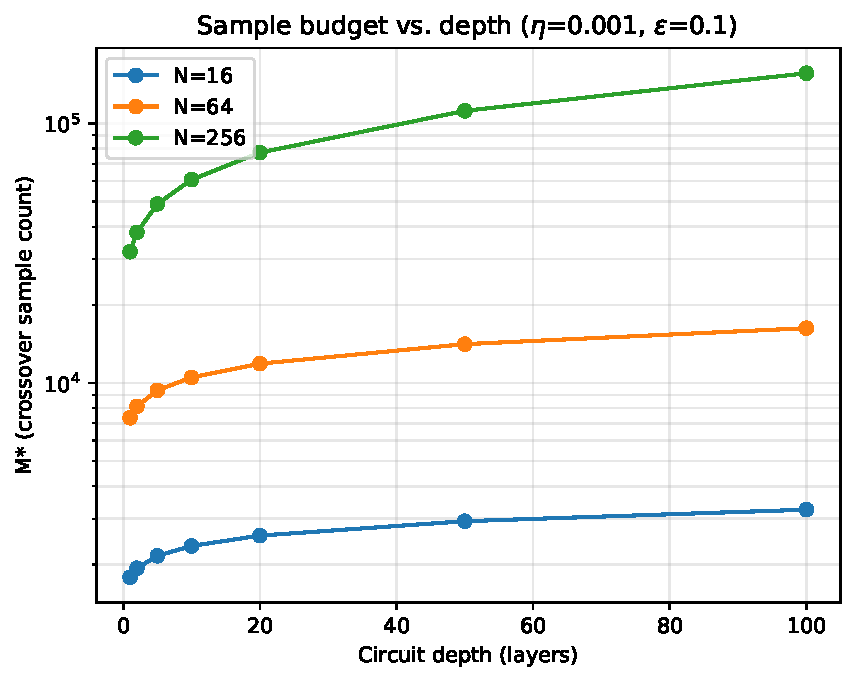
\includegraphics[width=0.48\textwidth]{../../results/figures/circuit_depth.pdf}
  \caption{Left: depolarizing-noise robustness (TVD vs.\ $\eta$).
  Right: circuit-depth crossover (samples vs.\ depth at fixed $\eta$).}
  \label{fig:noise-depth}
\end{figure}

\subsection{Real dataset classification (Zhao et al.\ replication)}
The notebook \texttt{real\_datasets\_colab.ipynb} reproduces the six-dataset
suite from Zhao et al.\ (2026): IMDb, 20 Newsgroups, PBMC3k, PBMC68k,
Dorothea, and Splice.  Each dataset emits machine-size vs.\ accuracy and
variance-recovery curves.  PBMC68k uses the full $\sim$68k-cell download via
\texttt{scvelo} (cached locally); see \texttt{load\_pbmc68k()} in the package.

Warmstart ablation numbers for the K-sparse regime are tabulated in
\texttt{results/tables/table\_warmstart\_ablation.tex} (generated by
\texttt{scripts/generate\_paper\_tables.py}).
